\chapter{Other \label{chap:otherappendices}}


\section{Useful Links}
Sample generated animations and animations used in the questionnaire: \videoshost \newline
The Emotional Body Motion Database: \url{http://ebmdb.tuebingen.mpg.de/} \newline
IBM Watson Tone Analyzer: \url{https://www.ibm.com/watson/services/tone-analyzer/} \newline
Tone Analyzer Guide: \url{https://console.bluemix.net/docs/services/tone-analyzer/} \newline
Blender: \url{http://www.blender.org/} \newline
International Movie Script DataBase: \url{http://www.imsdb.com} \newline
DB browser for Sqlite: \url{ttp://www.sqlitebrowser.org} \newline


\section{The questionnaire \label{sec:appquestionnaire}}
Please see figures ~\ref{fig:firstquestionnaire} to ~\ref{fig:lastquestionnaire}.


\begin{figure}[h]
	\makebox[\textwidth][c]{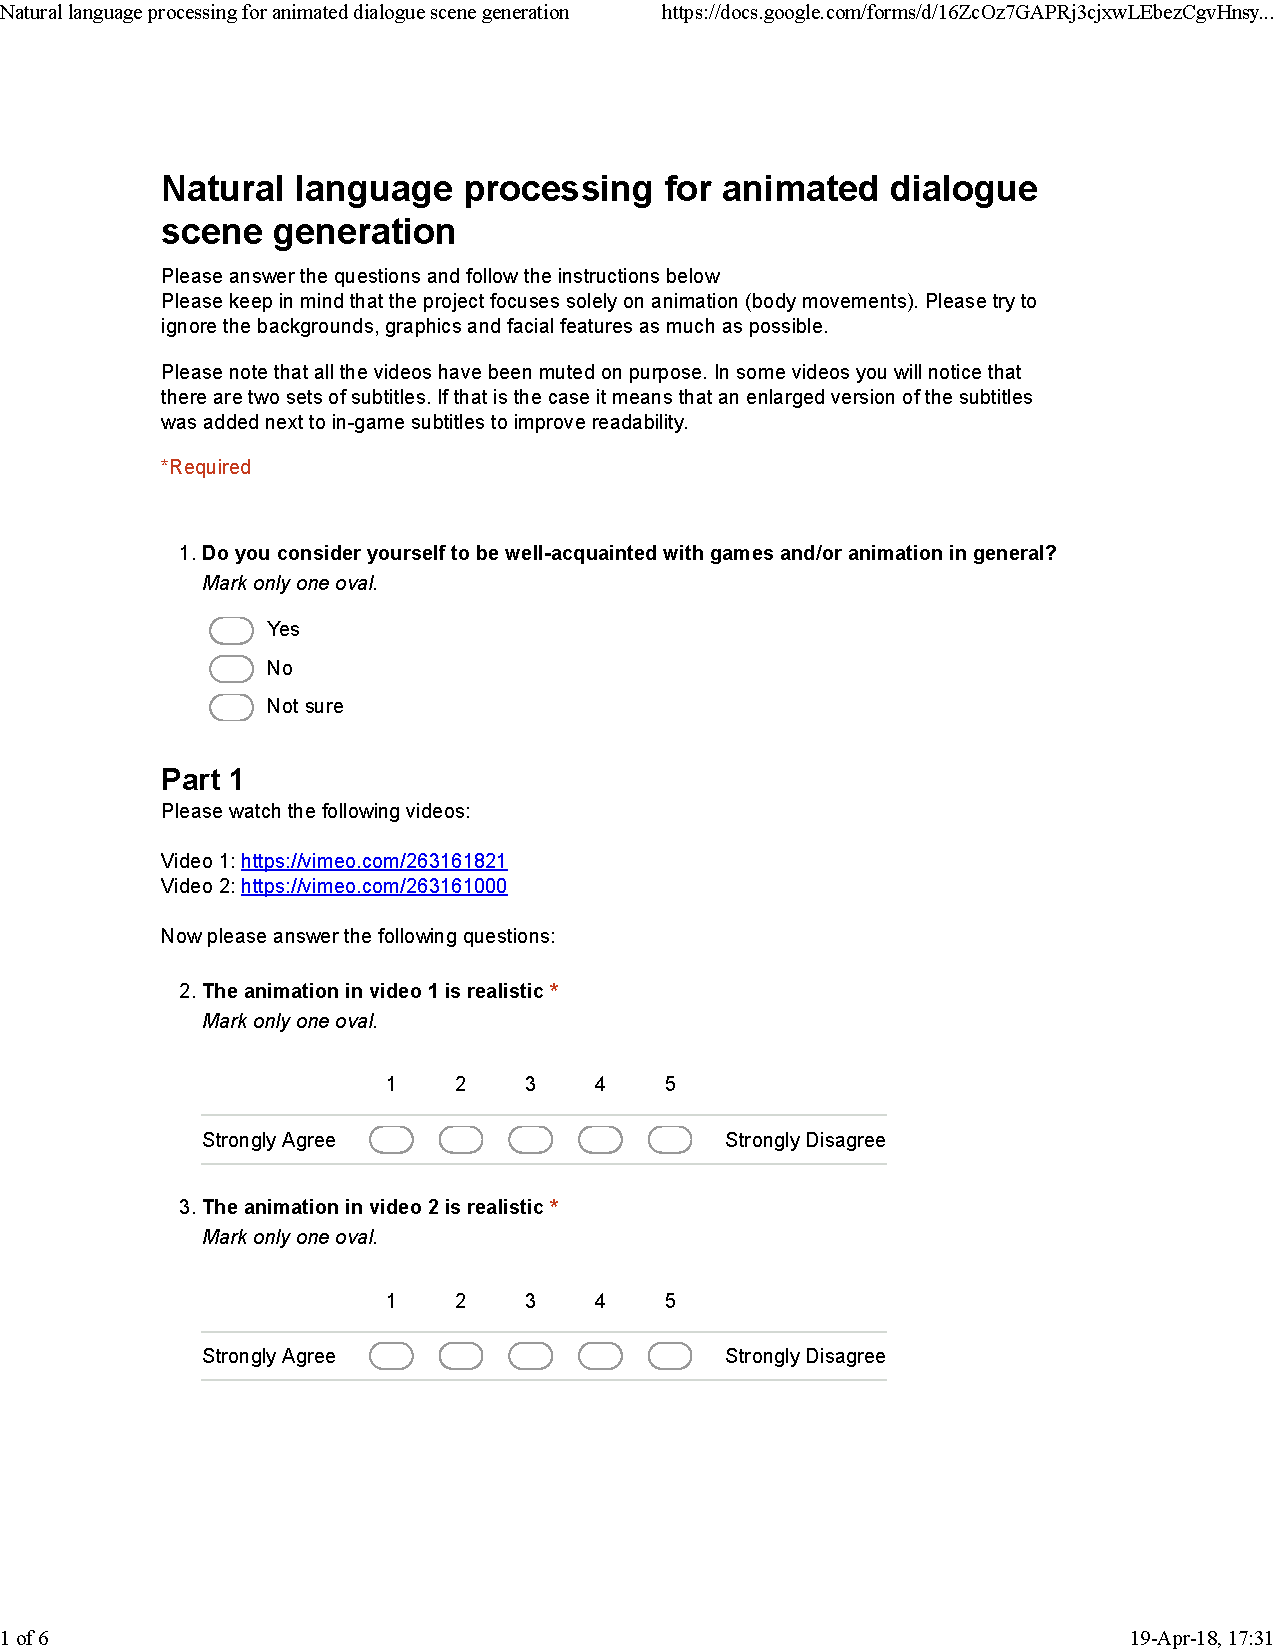
\includegraphics[page=1,width=1.2\textwidth]{img/appendix/questionnaire.pdf}}
	\caption{The questionnaire - page 1}\label{fig:firstquestionnaire}
\end{figure}

\begin{figure}[h]
	\makebox[\textwidth][c]{\includegraphics[page=2,width=1.2\textwidth]{img/appendix/questionnaire.pdf}}
	\caption{The questionnaire - page 2}
\end{figure}

\begin{figure}[h]
	\makebox[\textwidth][c]{\includegraphics[page=3,width=1.2\textwidth]{img/appendix/questionnaire.pdf}}
	\caption{The questionnaire - page 3}
\end{figure}

\begin{figure}[h]
	\makebox[\textwidth][c]{\includegraphics[page=4,width=1.2\textwidth]{img/appendix/questionnaire.pdf}}
	\caption{The questionnaire - page 4}
\end{figure}

\begin{figure}[h]
	\makebox[\textwidth][c]{\includegraphics[page=5,width=1.2\textwidth]{img/appendix/questionnaire.pdf}}
	\caption{The questionnaire - page 5}
\end{figure}

\begin{figure}[h]
	\makebox[\textwidth][c]{\includegraphics[page=6,width=1.2\textwidth]{img/appendix/questionnaire.pdf}}
	\caption{The questionnaire - page 6}\label{fig:lastquestionnaire}
\end{figure}



\section{Sample generated scene used in the questionnaire \label{sec:samplescene}}
The following scene comes from the game \textit{Horizon: Zero Dawn}. The screenshots depicting the scene can be found in figures ~\ref{fig:screenshotfirst} to ~\ref{fig:screenshotlast}. Please note that the top images represent the original scene while the bottom ones show the recreated scene. 


\begin{figure}[h]
	\centerline{\fbox{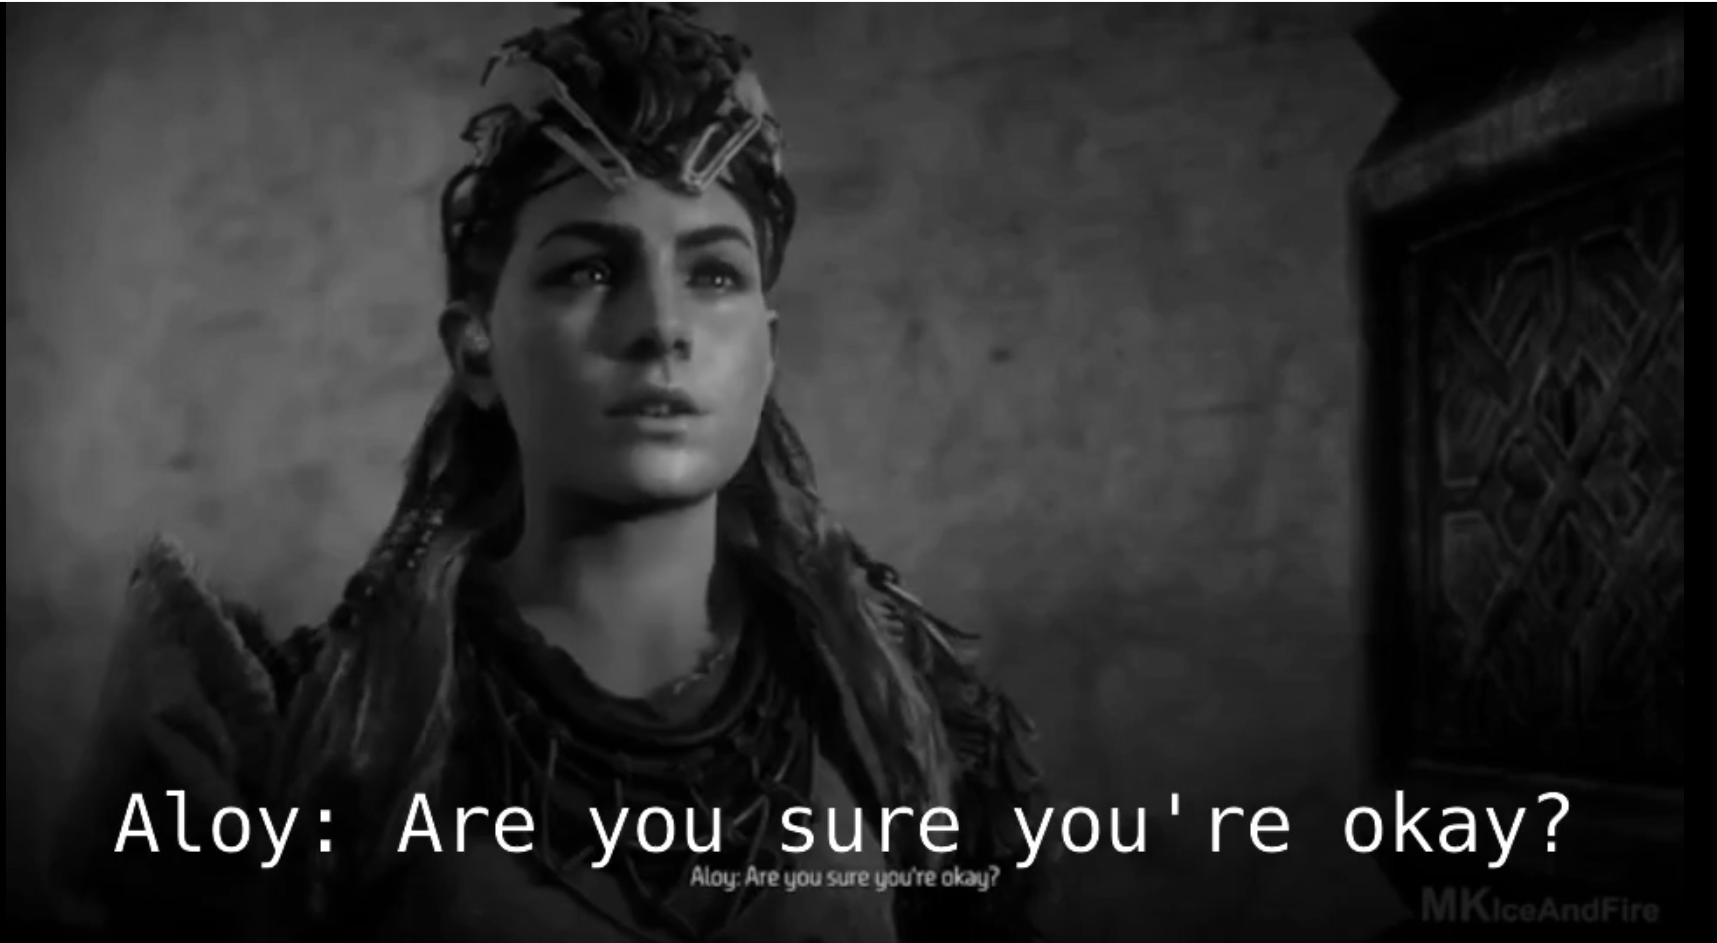
\includegraphics[width = 30em]{img/appendix/sample/horizon1.png}}}
	\centerline{\fbox{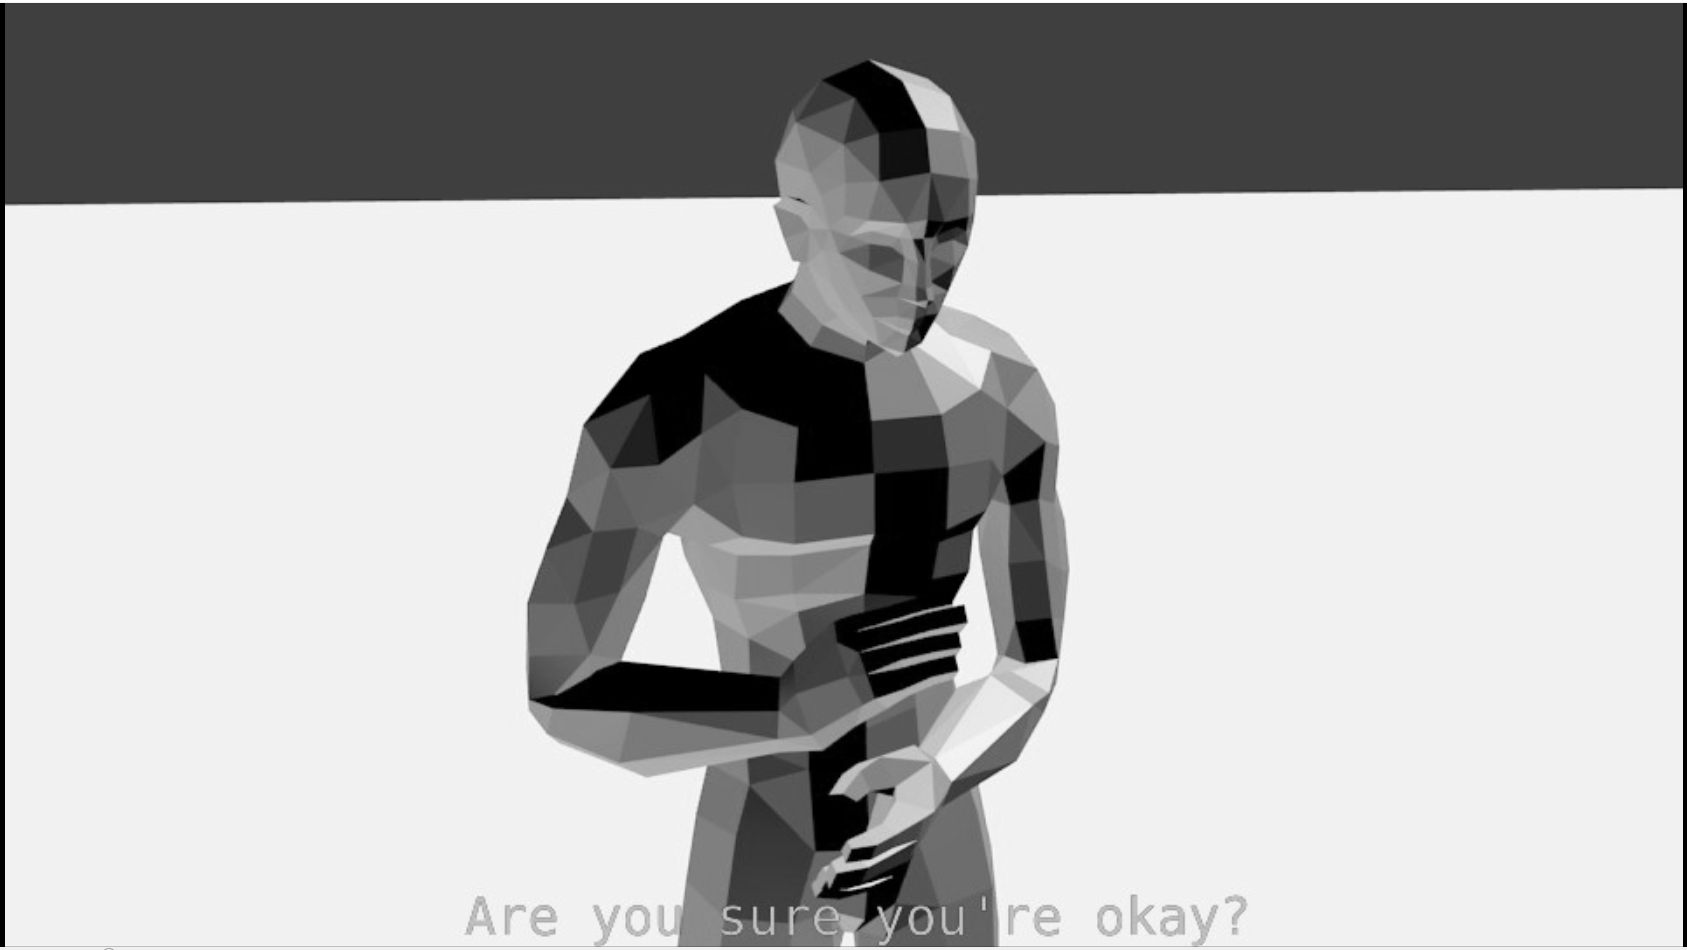
\includegraphics[width = 30em]{img/appendix/sample/horizonrender1.png}}}
	\caption{Dialogue line 1. \\ Transcript: `Aloy: Are you sure you're okay?'}\label{fig:screenshotfirst}
\end{figure}

\begin{figure}[h]
	\centerline{\fbox{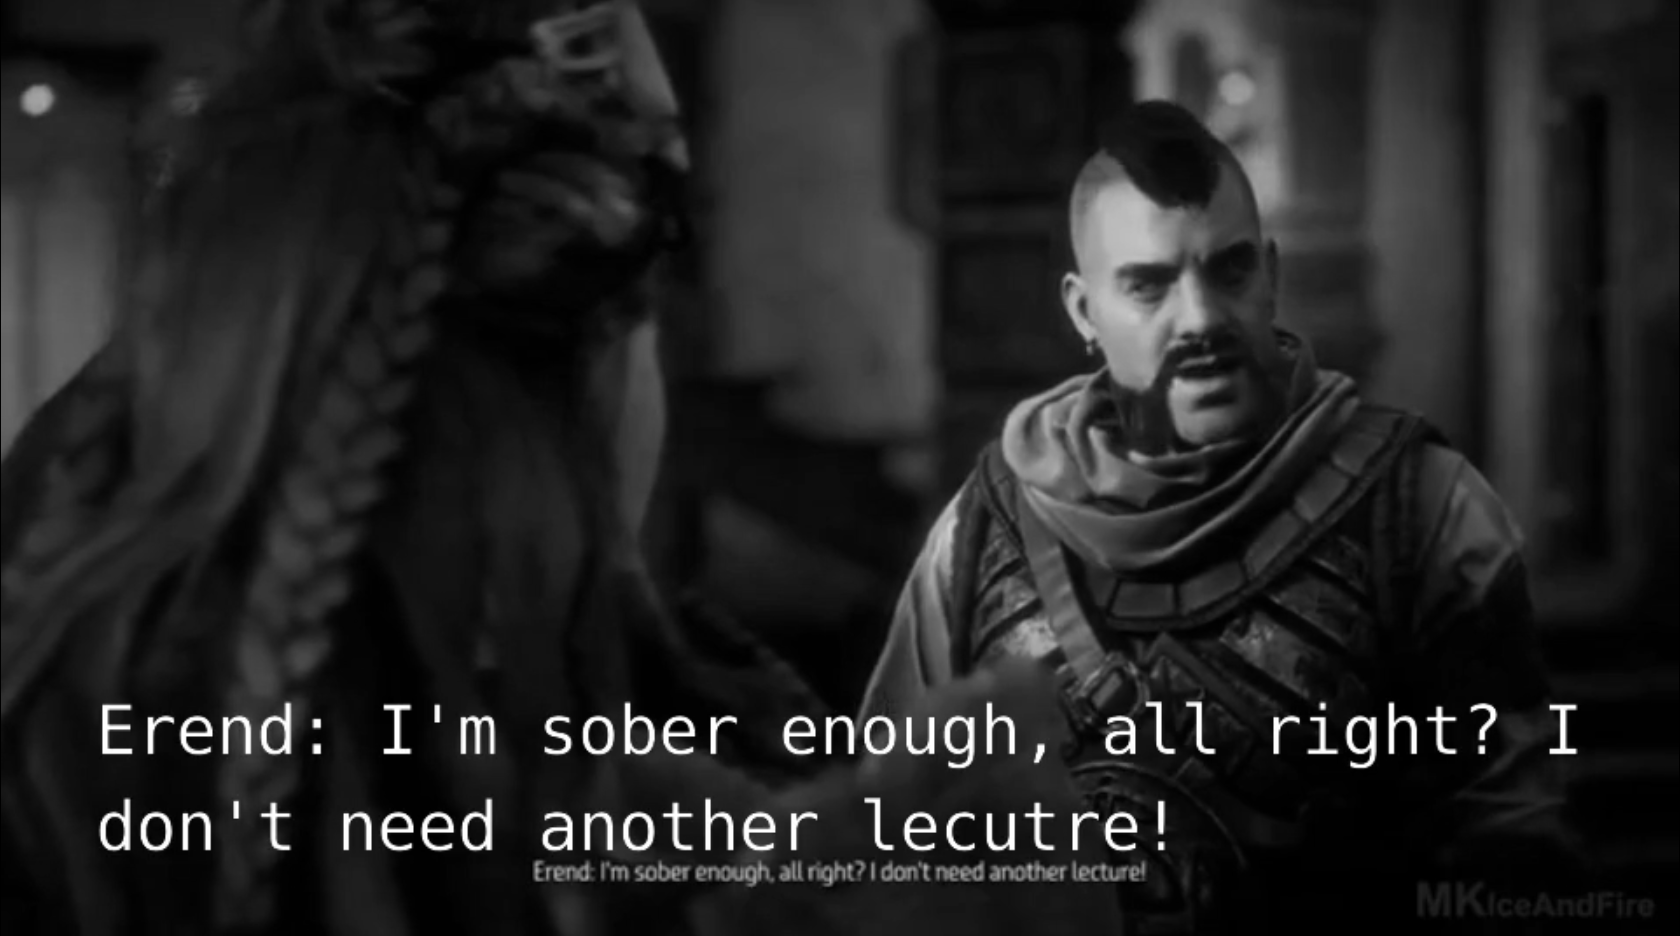
\includegraphics[width = 30em]{img/appendix/sample/horizon2.png}}}
	\centerline{\fbox{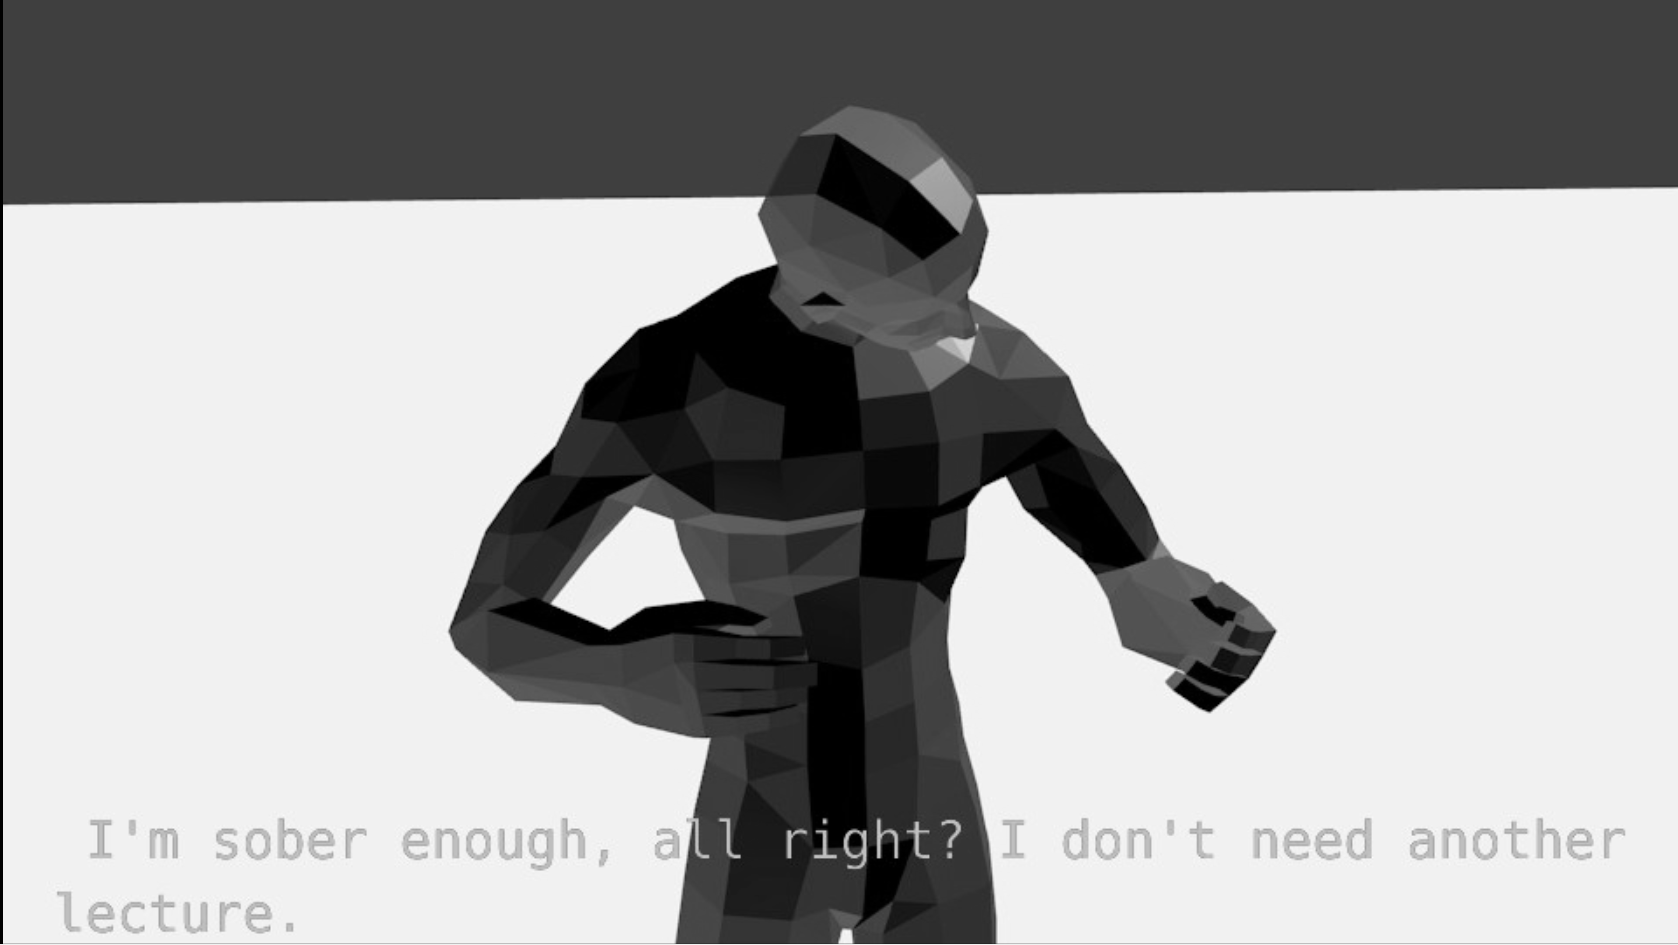
\includegraphics[width = 30em]{img/appendix/sample/horizonrender2.png}}}
	\caption{Dialogue line 2. \\ Transcript: `Erend: I'm sober enough, all right? I don't need another lecture!'}
\end{figure}

\begin{figure}[h]
	\centerline{\fbox{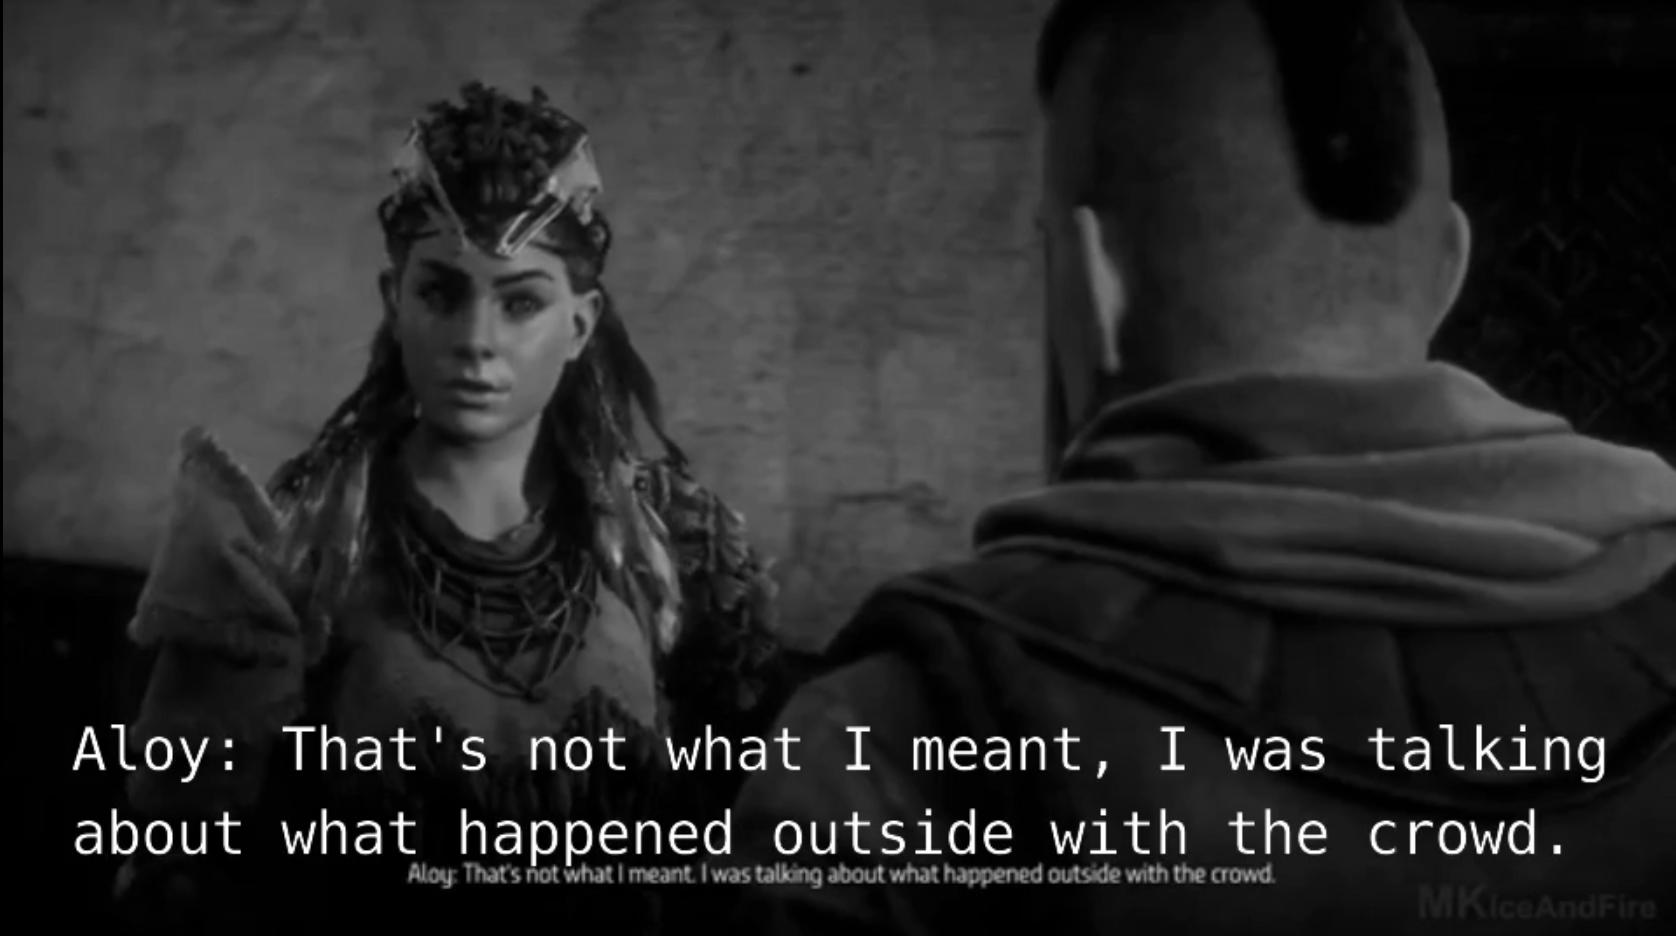
\includegraphics[width = 30em]{img/appendix/sample/horizon3.png}}}
	\centerline{\fbox{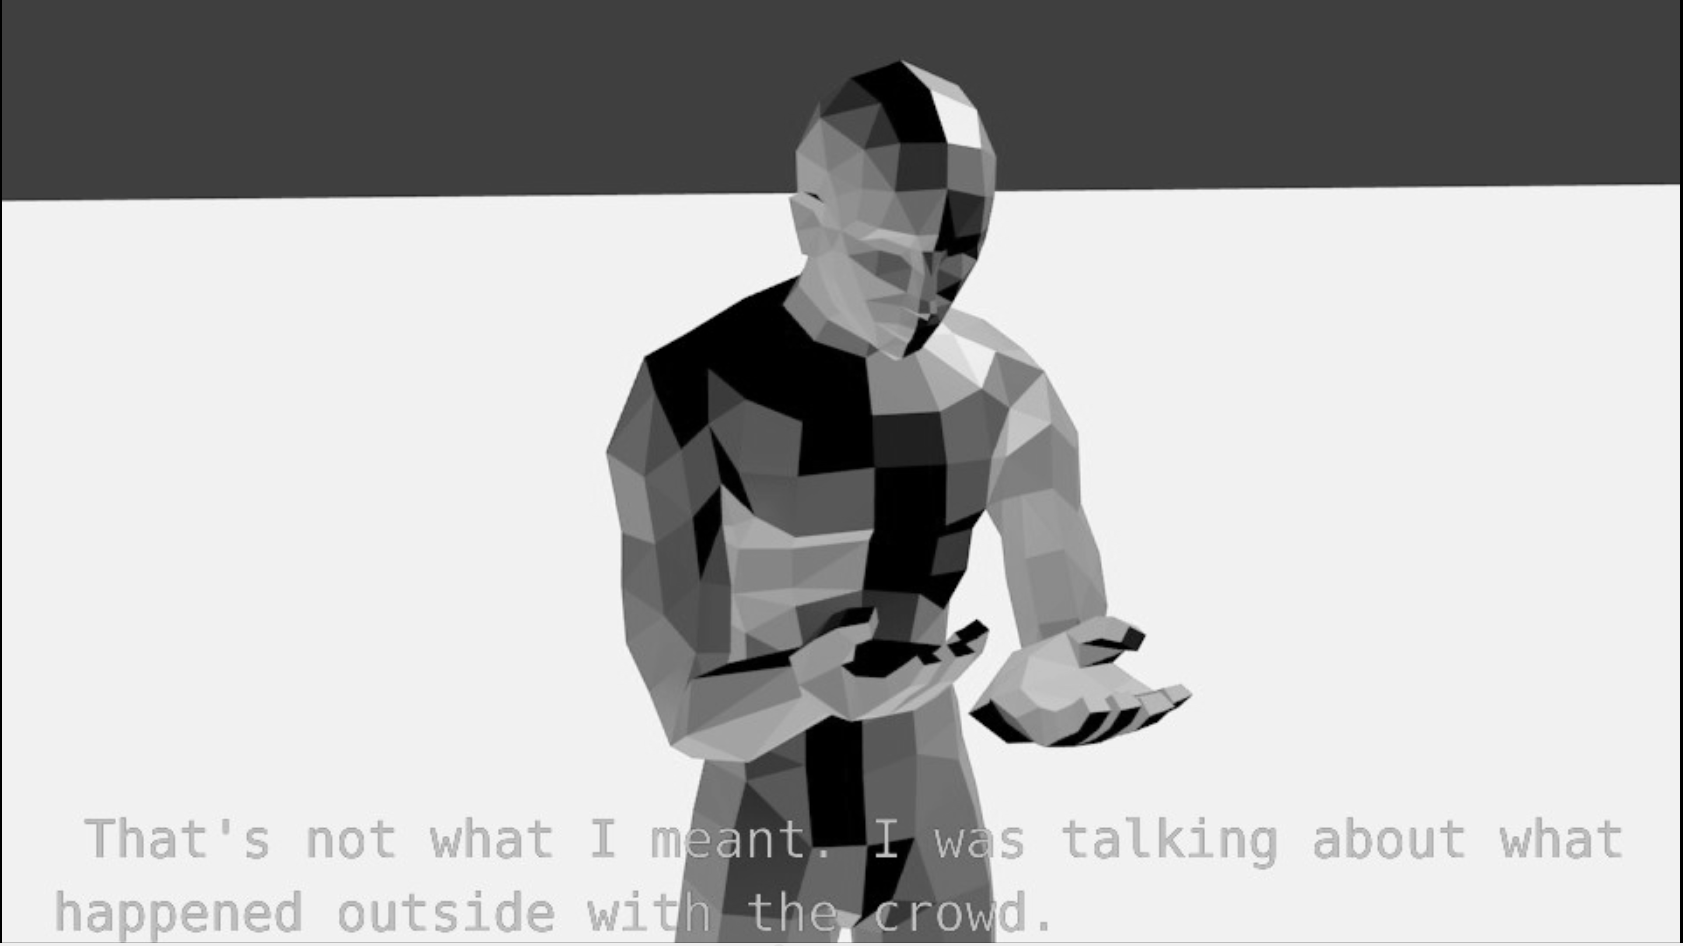
\includegraphics[width = 30em]{img/appendix/sample/horizonrender3.png}}}
	\caption{Dialogue line 3. \\ Transcript: `Aloy: That's not what I meant, I was talking about what happened outside with the crowd.'}
\end{figure}

\begin{figure}[h]
	\centerline{\fbox{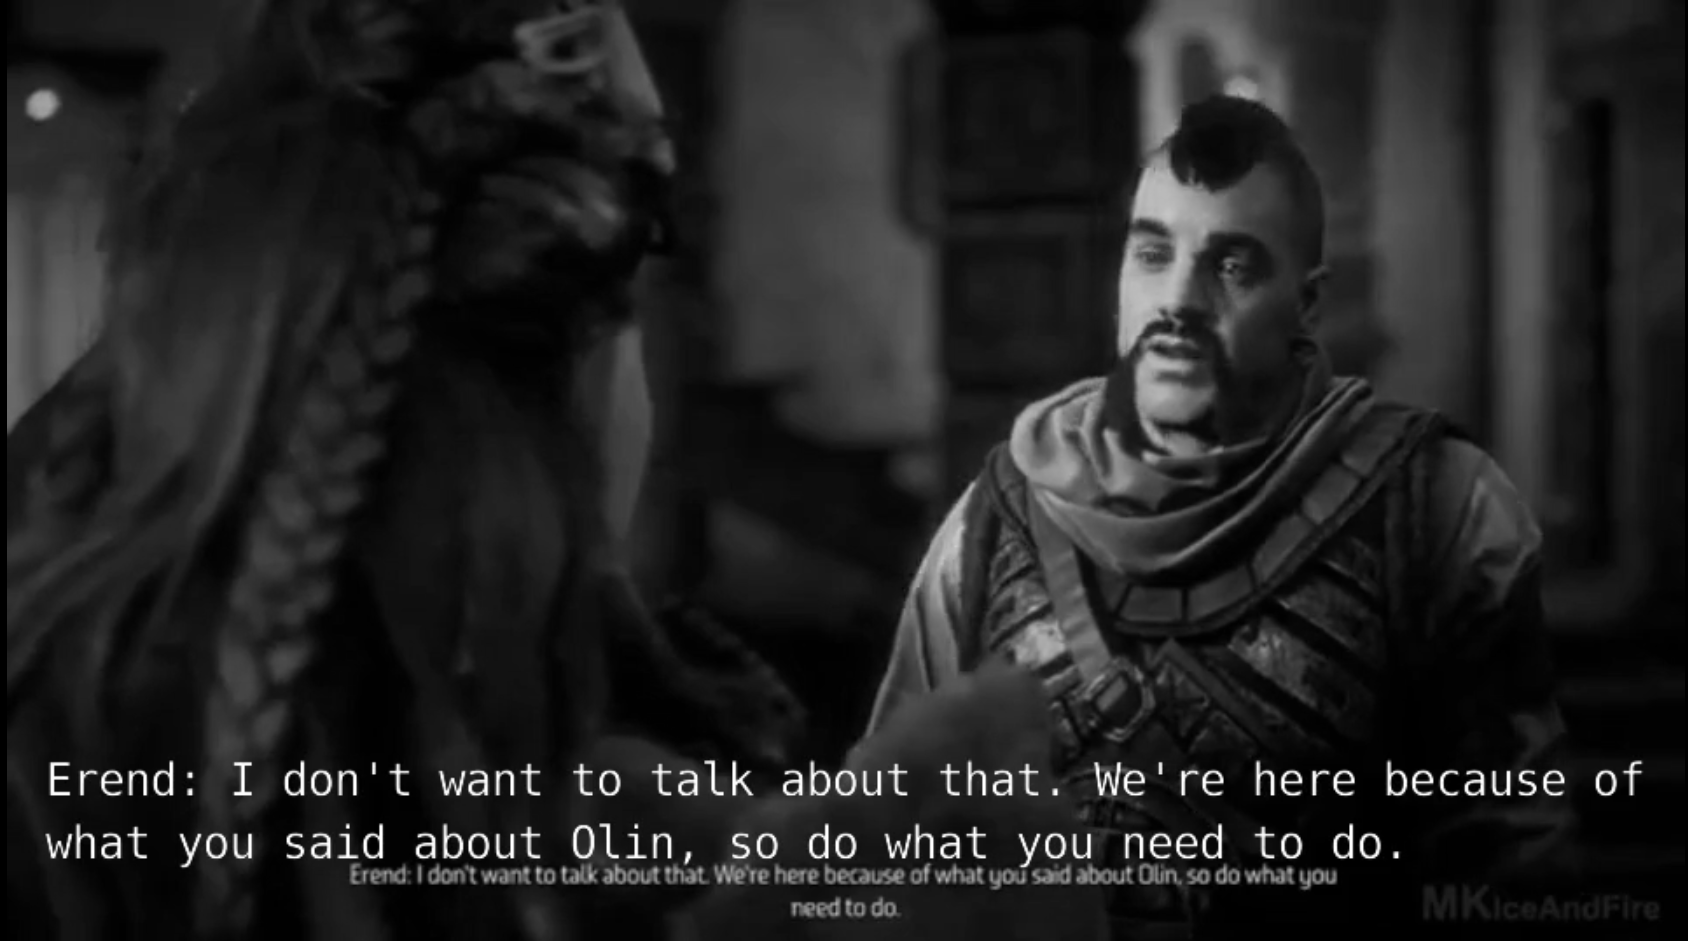
\includegraphics[width = 30em]{img/appendix/sample/horizon4.png}}}
	\centerline{\fbox{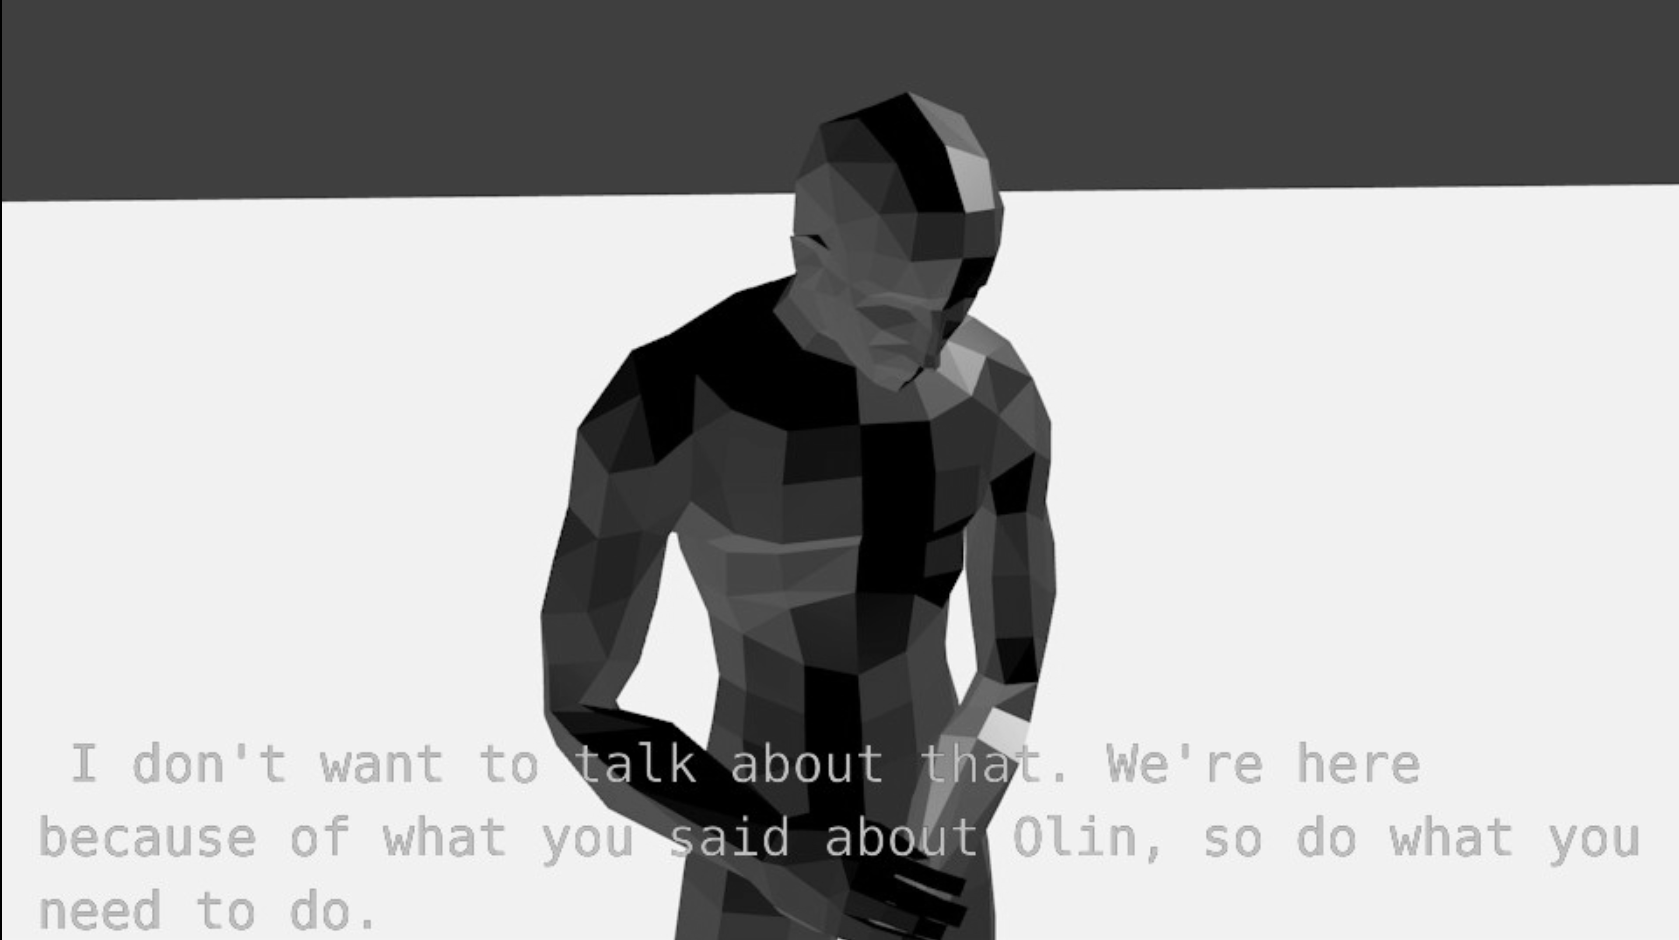
\includegraphics[width = 30em]{img/appendix/sample/horizonrender4.png}}}
	\caption{Dialogue line 4. \\ Transcript: `Erend: I don't want to talk about that. We're here because of what you said about Olin, so do what you need to do.'}\label{fig:screenshotlast}
\end{figure}


\section{Interviewees' comments about the recreated animations \label{sec:qcomments}}
The following is a full list of comments that the interviewees made when asked to justify some of their choices. Those comments were not required of the participants and some refused to give more detailed feedback. Please note that Animation/Option/Video 1 refers to the original animation, while the Animation/Option/Video 2 refers to the recreated one.

\noindent Comments in favour of the recreated animations:
\begin{itemize}
	\item `The second animation is corresponding better to the situation in the game.'
	\item `Active body language refers to what is being said.'
	\item `Better expression of emotions but sometimes they were exaggerated.'
	\item `Both animations present natural movements of the body.'
	\item `No body language [in animation 1].'
	\item `More accurate expression of feelings.'
	\item `Option 2 because character has more natural behavior.'
	\item `Body language matches with what is being said.'
	\item `Natural body motions [in animation 2].'
\end{itemize}

\noindent Comments in favour of the original animations:
\begin{itemize}
	\item `Weird hands movement in the 2nd one.'
	\item `Option 1 because in option 2 author moved too far.'
	\item `Weird hand movement in the 2nd one.'
	\item `[Animation 1] Looks better.'
\end{itemize}


\noindent Other comments:
\begin{itemize}
	\item `Both about the same, animation 1 didnt represent any emotion, animation 2 was little over the top'
	\item `Both animation represented the scene about the same, didnt really have a preference.'
	\item `I think both represented the emotion about the same.'
	\item `Option 1 is not bad, option 2 is overly exaggerated.'
\end{itemize}



